%!TEX root = ../../../adrien_gomar_phd.tex


\begin{figure}[htp]
  \centering
  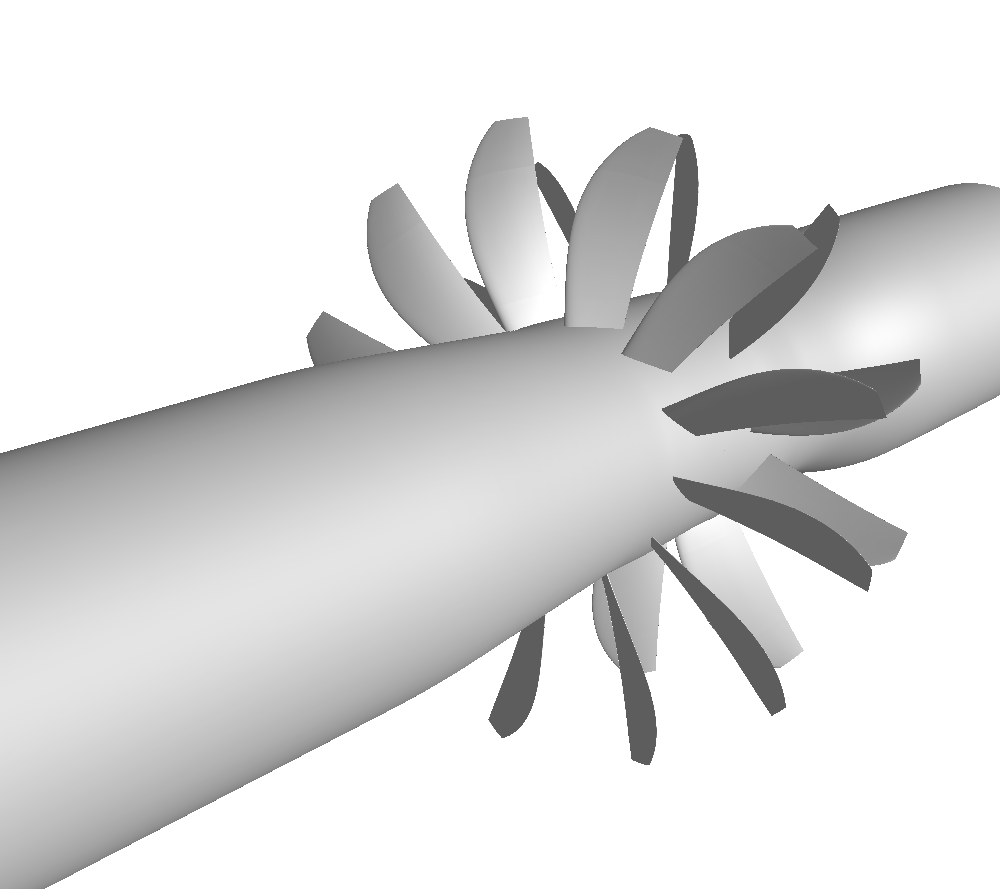
\includegraphics[width=.3\textwidth]{DREAM_LS_wall.png}
  \caption{Low-speed isolated contra-rotating open rotor geometry.}
  \label{fig:dream_ls_wall}
\end{figure}

The studied configuration is a pusher contra-rotating open rotor
that comes from the know-how of SAFRAN-Snecma. 
It is shown in Fig.~\ref{fig:dream_ls_wall} for the
Low-speed (LS) flight condition, representative of the take-off
and landing.
The simulated configuration does not include the spinner as the
experimental setup does not take into account this part of the geometry.
Sadly, the experimental results were not available for comparison
at the time this study was written.

\begin{table}[htp]
  \ra{1.3} \centering
  \begin{tabular}{cccc}
    \toprule
    $M_0$ & $|\Omega|$ & $J$ & $M_{tip}$ \\
    \midrule
    $0.2$ & $5739$ RPM & 1.06 & 0.63 \\
    \bottomrule
  \end{tabular}
  \caption{Low-speed isolated contra-rotating open rotor flight condition parameters.}
  \label{tab:dream_ls_flight_condition}
\end{table} 
Table~\ref{tab:dream_ls_flight_condition} recalls the main
parameters of the case: the inflow Mach number $M_0$,
the absolute value of the rotation speed of both rotors $|\Omega|$,
the advance ratio $J$ (whose definition is given in Chap.~\ref{cha:cror})
and the Mach number at the tip of
the front rotor blades based on the inflow velocity and the advance ratio:
\begin{equation}
	M_{tip} = M_0 \sqrt{1 + \left(\frac{\pi}{J} \right)^2}
  \label{eq:m_tip}
\end{equation}
Equation~\ref{eq:m_tip} is actually a simple transcription of the velocity triangle
applied to the infinite velocity and to the rotation speed perceived
at the front blade tip:
\begin{equation}
    M_{tip} = M_0 \sqrt{1 + \left(\frac{\pi}{J}\right)^2} = 
    \frac{V_0}{\sqrt{\gamma R t_0}} \sqrt{1 + \left(\frac{
    	\cancel{\pi} \cdot \Omega D}{
    	2 \cancel{\pi} \cdot V_0}\right)^2} =
    \sqrt{\frac{V_0^2 + (\Omega R)^2}{\gamma R t_0}}
    \label{eq:m_tip_explained}
\end{equation}

At this flight condition, the inflow Mach 
number $M_0$ is within the incompressible range
($M_0 < 0.3$). As the CFD flow solver used here is 
\textit{elsA}~\cite{Cambier2013} CFD code which is a compressible code, 
a preconditionner might be needed for the computations to converge. 
Hopefully, the fluid is accelerated by the two rotors
and the tip Mach number is high enough to not use any preconditionning.
However, let us bare in mind that this range of Mach number might
be tedious for a compressible flow solver.
The advance ratio $J$ is around~1 which is a classical value for
low-speed propellers~\cite{Bousquet2012}. Note that the rotation speed is almost
one order of magnitude larger than expected. 
In fact, a full-scale CROR diameter is around 5~meters. With this rotation speed
($|\Omega|=5739~RPM$),
this would lead to a tip Mach number greater than~4. This high rotation speed is 
actually here to compensate for the small radius of the blades 
while maintaining the same similarity coefficients. It i
is actually 33~cm for experimental purposes.

Two structural modes are considered for the aeroelastic study of this 
configuration: the second bending/flexion mode and the first torsion mode
of the front rotor. These were inputs of the current work.
The shape of the modes is shown in Fig.~\ref{fig:dream_ls_ael_modes}
with an arbitrary amplitude, large enough to ease the visualization.
Two inflection lines are seen for the 2F mode, while only
one is seen for the 1T, hence their designation.
\begin{figure}[htp]
  \centering
  \subfigure[2F]{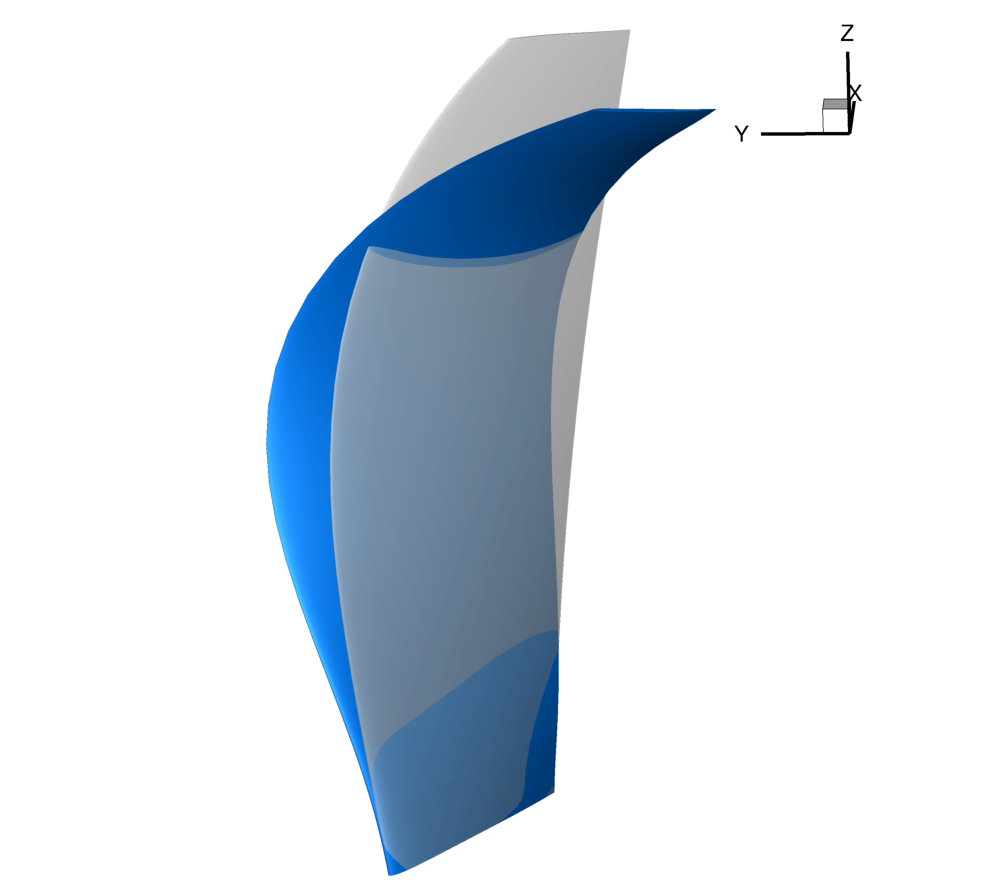
\includegraphics[height=.35\textwidth]{mode_2F.png}}
  \subfigure[1T]{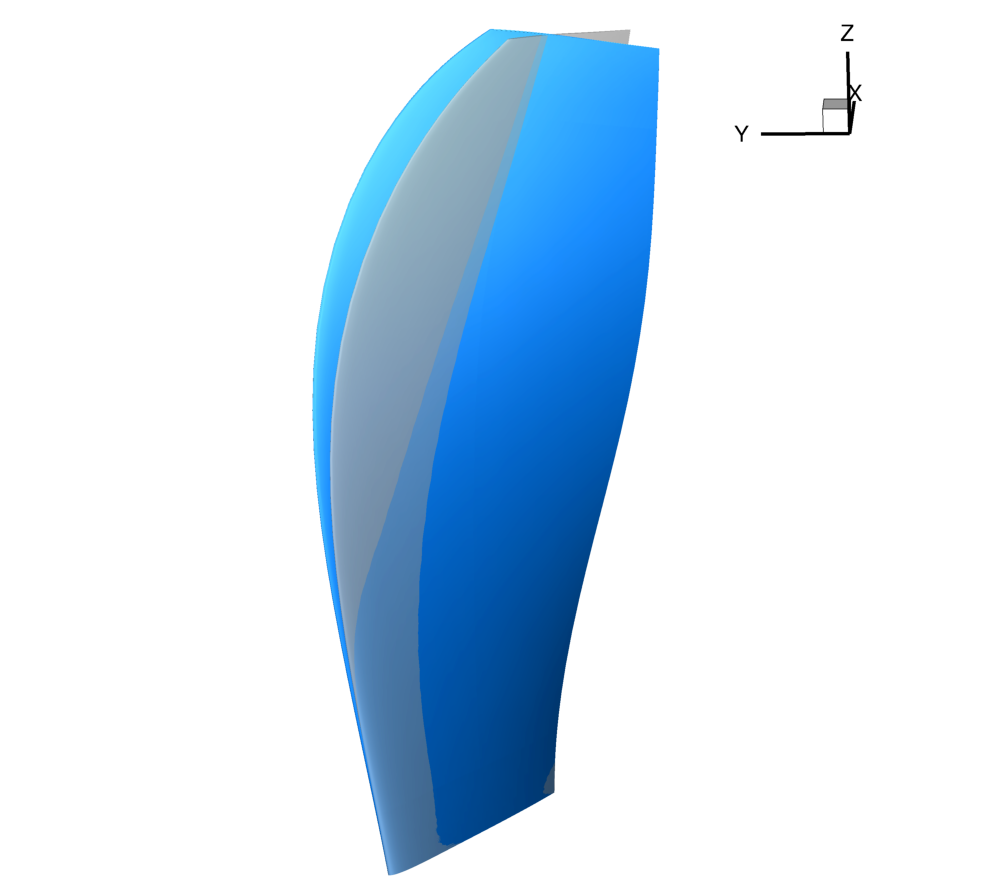
\includegraphics[height=.35\textwidth]{mode_1T.png}}
  \caption{Low-speed isolated configuration: structural modes considered.}
  \label{fig:dream_ls_ael_modes}
\end{figure}
The frequency, mass and stiffness of the modes 
are given with the corresponding modes.
The frequency of each mode vary between 
$495~\textrm{Hz} \leq f_{AEL} \leq 600~\textrm{Hz}$
while the blade passing frequency of the opposite rows,
namely the rear rotor, is $1913~\textrm{Hz}$. However,
this last frequency governs the unsteady rigid flow physics 
and will have to be computed along with the aeroleastic frequency.
Therefore, the multi-frequential formulation of the
harmonic balance approach will be used to simulate the
aeroelastic response of the blades (see Sec.~\ref{sec:dream_ls_ael_results}).
